\chapter{Multiple use: Anonymity with Non-linkability}
\label{chap:mult}
Here we describe three solutions for anonymous threshold signature schemes with non-linkability property.

\section{Constant Size Anonymous Threshold Signature}

\citeauthor*{DazaDSV09} proposed in \cite{DazaDSV09} an anonymous threshold signature scheme that sets a $(t,r)$-threshold signature scheme based on Shamir's secret sharing over a partition of the set $\PP$ of participants.

\subsection{Description}
\label{sec:daza}
\subsubsection*{Setup Algorithm}
\begin{itemize}[align = left, leftmargin=*, label={--}]
\item Let $\PP = \{P_1 , \dots , P_n \}$ be the set of participants. Consider $d$ distinct partitions of $\PP$ into $r$ parts.
$\PP^i = \{\PP^i_1, ... , \PP^i_r\}$ for $i \in \{1, ... , d\}$. This algorithm will set $d$ different threshold signature schemes, one for each partition of $\PP$.

\item Let $p > n$ be a sufficiently large prime. Let $sk_i \in_R \ZZ_p$ be the secret key of the $i$-th threshold signature scheme. Let $P_i(x)$ be a random polynomial over $\ZZ_p$ of degree $t-1$ with ${P_i(0) = \mbox{sk}_i}$ for $i \in \{1, ..., d\}$.

\item For $i \in \{1, ..., d\}$ let $\alpha^{(i)}_1, ... , \alpha^{(i)}_r \in_R \ZZ_p$ all distinct (for fixed $i$). Each participant $P_k \in \PP^i_j$ is given public key $pk^{(i)}_k = \alpha^{(i)}_j$ and secret key $sk^{(i)}_k = P_i(\alpha^{(i)}_j)$ for the $i$-th threshold signature scheme. 
\end{itemize}

\subsubsection*{Signing Algorithm}
\begin{itemize}[align = left, leftmargin=*, label={--}]
\item Let $\{P_{i_1}, ..., P_{i_t} \} \subseteq \PP$ a set of $t$ participants which will try to sign a message $m$.

\item A signature on $m$ over the $i$-th threshold signature scheme is attempted using the protocol described in section \ref{sec:shamir_sig} providing the message, the signature and the signature scheme over which is signed: $(m,\sigma, i)$.

\item If the signature fails (because $\alpha^{(i)}_{i_1}, ... , \alpha^{(i)}_{i_t}$ are not all distinct), a new signature on $m$ is attempted over a threshold signature scheme different from the previous tried.

\item Eventually, the signature will succeed over a certain signature scheme.
\end{itemize}

\subsubsection*{Verifying Algorithm}
\begin{itemize}[align = left, leftmargin=*, label={--}]
\item Let $(m, \sigma, i)$ be a signature on a message $m$. The verification is done using the verifying algorithm described in \ref{sec:shamir_sig}.
\item Let $e$ be a bilinear pairing. The signature is valid if and only if $e(\sigma,g) = e(H(m),pk_i)$.
\end{itemize}

\subsection{Analysis}
In this signature scheme it is not sure that any set of $t$ participants will be able to compute a signature on a given message. The probability of succeeding on signing a message depends on the parameters $t,n,r,d$ and how the partitions are made.

To see the relation between these parameters and the probability of success, we will describe a few examples.

Given $\{P_{i_1}, ... P_{i_t} \}$ a set of $t$ participants, they will succeed only if $\alpha^{(i)}_{i_1}, ..., \alpha^{(i)}_{i_t} $ are all distinct for a certain $i \in \{1, ...,d\}$. Hence, $t \leq r$.

\subsubsection*{Random partitions}
Suppose that for each participant $P_k \in \PP$ and for all $i \in \{1, ..., d\}$ the probability $Pr(P_k \in \PP^i_j) = \frac{1}{r}$ holds.

The probability that, given $t$ participants, they succeed on signing a message in the $i$-th threshold signature scheme (i.e. no two participants share the same public key) is given by $p_{succ,i} = \prod_{k=0}^{t-1} (1-\frac{i}{r}) = 1 - \frac{t(t-1)}{2r} + o\left( \frac{t^2}{r} \right)$

Thus, the probability of failing to sign a message in the $i$-th threshold signature scheme is $p_{fail,i} = 1 - p_{succ,i} = \frac{t^2}{2r} + o\left( \frac{t^2}{r} \right)$.

The global probability of failing to sign a message is $p_{fail} = \prod_{i=1}^d p_{fail,i} = {\left(\frac{t^2}{2r}\right)^d + o\left( \left( \frac{t^{2}}{r} \right)^d \right)}$

\begin{table}[H]
\begin{center}
    \begin{tabular}{|c|r|c|r|r|c|}
        \hline
        $\frac{t^2}{2r}$ & \multicolumn{1}{c|}{$t$} & $\frac{n}{r}$ & \multicolumn{1}{c|}{$n$} & \multicolumn{1}{c|}{$r$} & $p_{fail}$ \\ \hline
        
        \multirow{4}{*}{$10^{-3}$} & $5$ & \multirow{4}{*}{$10^{3}$} & $12.5 \cdot 10^6$ & $12.5 \cdot 10^{3}$ & $0.80 \cdot 10^{-3}$ \\ \cline{2-2} \cline{4-6}
        & $10$ & & $50 \cdot 10^6$ & $50 \cdot 10^{3}$ & $0.90 \cdot 10^{-3}$ \\ \cline{2-2} \cline{4-6}
        & $50$ & & $1.25 \cdot 10^9$ & $1.25 \cdot 10^{6}$ & $0.98 \cdot 10^{-3}$ \\ \cline{2-2} \cline{4-6}
        & $100$ & & $5 \cdot 10^9$ & $5 \cdot 10^{6}$ & $0.99 \cdot 10^{-3}$ \\ \cline{2-2} \cline{4-6}
        
        \hline

    \end{tabular}
\end{center}
\caption{Sample values for $p_{fail,i}$}
\end{table}


\subsubsection*{Deterministic partitions}


To simplify the analysis, for each participant $P_k \in \PP$ we will consider the corresponding codeword in a (not necessary linear) code of length $d$ over an alphabet of size $r$ given by:
$$c_k := (j_1, ... , j_d) \text{ iff } P_k \in \PP^i_{j_i} \quad \forall i \in \{1, ..., d\}$$

\begin{thm}[Singleton \cite{singleton}]
Let $C$ be a code of length $n$, minimum distance $d$ over an alphabet of size $q$ and cardinality $M$. The cardinality is upper bounded by $\log_q M \leq n-d+1$.
\end{thm}

Changing the notation to adapt it to our case, if we want all codewords associated to the participants to be different, we have $log_r n \leq d - \delta + 1$ where $\delta$ would be the minimum distance of the code (i.e. the least number of schemes that any two participants have distinct public keys in them). For $\delta \geq 1$ we have $n \leq r^d$.

It is reasonable to wonder whether it is possible or not to define $d$ partitions of $\PP$, such that any set of $t$ participants lie in different parts of a certain partition $\PP^i$. To answer that question, we need the following definition.

\defn Let $m \geq w \geq 2$. An $(n,m,w)$-perfect hash family is a set of functions $\F$ where $\card{Y} = n$, $\card{X} = m$ and $f: Y \rightarrow X$ for each $f \in \F$, such that, for any $C \subseteq Y$ with $\card{C} = w$, there exists at least one function $f \in \F$ such that $f \vert_C$ is one-to-one. When $\card{\F} = N$, an $(n,m,w)$-perfect hash family will be denoted by \textbf{PHF}$(N;n,m,w)$.

Getting back to our question: let $Y = \PP$, $X = \{1, ..., r\}$ and let $\F = \{f_1, ..., f_d\}$ where $f_i(P_k) = (c_k)_i$. It is possible to define $d$ partitions of $P$ in a way that any set of $t$ participants lie in different parts of a certain partition $P^i$ if and only if there exists a \textbf{PHF}$(d;n,r,t)$. PHF exist only for suitable sets of values for the parameters. The following theorem gives a (not tight) lower bound on $\card{\F}$ s.t. there exists a PHF.

\begin{thm}[2.1 \cite{Deng04}]
There exists a \textbf{PHF}$(d;n,r,t)$ if
$$ d > \frac{\log \binom{n}{t}}{\log r^t - \log (r^t - t! \binom{r}{t})} $$
\end{thm}

\begin{figure}[H]
    \begin{center}
        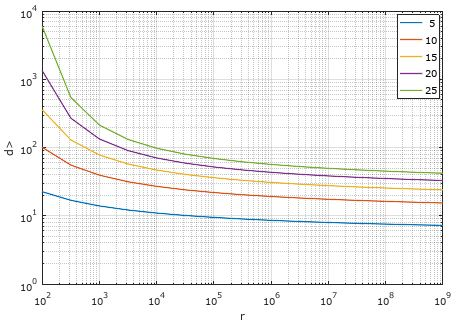
\includegraphics[scale=1.5]{images/phf.jpg}
    \end{center}

    \caption{Lower bound of $d$ for different values of $t$ with $\frac{n}{r} = 10^3$}
    \label{fig:phf} 
\end{figure}

The plot in Figure \ref{fig:phf} gives a hint that the bound might have limit when $r \rightarrow \infty$ fixing $\frac{n}{r}=c$ constant. Note that $r^t - t! \binom{r}{t} = \frac{t(t-1)}{2}r^{t-1} + o(r^{t-1})$ for fixed $t$. Using the inequality $ \left( \frac{n}{t} \right)^t \leq \binom{n}{t} \leq n^t$ and the previous approximation for $r \gg t$, we have:
$$\frac{t \log \frac{n}{t}}{\log r + \log \frac{t(t-1)}{2}} \lesssim \frac{\log \binom{n}{t}}{\log r^t - \log (r^t - t! \binom{r}{t})} \lesssim \frac{t \log n}{\log r + \log \frac{t(t-1)}{2}}$$

Clearly, the limit when $r \rightarrow \infty$ and $n = c \cdot r$ ($c$ a constant), is $t$ on both sides of the inequality.

\section{Linkable Group Signature Scheme}
\label{sec:chen}
\citeauthor{ChenNW11} proposed a $(t,n)$-threshold signature scheme in \cite{ChenNW11} using a group signature scheme where you can link two signatures on the same message but cannot link signatures on different messages. As one can link signatures on the same message, the threshold signature is simply a set of $t$ valid signatures on the same message.
\subsection{Description}
\subsubsection*{Setup Algorithm}
\begin{itemize}[align = left, leftmargin=*, label={--}]
\item Let $G_1$, $G_2$, $G_T$ be cyclic groups of sufficiently large prime order $q$. Two random generators $g_1 \in G_1$, $g_2 \in G_2$, and a bilinear pairing $\hat{t}: G_1 \times G_2 \rightarrow G_T$.

DDH problem in $G_1$, Gap-DL problem in $G_1$ and $G_2$ and the blind bilinear LRSW problem are hard.

\item Let $H_0 : \{0,1\}^\ast \rightarrow \ZZ_q$ and $H_1 : \{ 0 , 1 \}^\ast \rightarrow G_1$ be two hash functions.

\item For each issuer $i \in \mathcal{I}$ the following is performed.

Two integers are selected $x,y \in_R \ZZ_q$ and the issuer secret key \textbf{isk} is assigned to be $(x,y)$. Then the values $X = g_2^{x} \in G_2$ and $Y = g_2^{y} \in G_2$ are computed. The issuer public key \textbf{ipk} is assigned to be $(X,Y)$.

\item The system public parameters $par$ are set to be $par = (G_1, G_2, G_T, \hat{t}, g_1, g_2, H_0, H_1, \text{ipk}_k)$ and are published.
\end{itemize}

\subsubsection*{Join protocol}
\begin{itemize}[align = left, leftmargin=*, label={--}]
\item In this a protocol, an issuer $i \in \mathcal{I}$ computes a credential for a signer $\s \in S$ that allows him to compute valid signatures on messages.

\item The signer $\s$ randomly chooses the secret key $sk_\s = f \in_R \ZZ_p$ and computes the public key $pk_\s = F = g_1^f$.

\item The issuer $\i$ randomly chooses $r \in_R \ZZ_q$ and computes $A = g_1^r$, $B = A^y$ and ${C = A^x F^{rxy}}$. The credential for $\s$ is set to be $cre_\s \leftarrow (A,B,C)$.
\end{itemize}

%\begin{figure}[H]
%$$
%\begin{array}{ccc}
%    \text{Signer}(\mathfrak{s}) &    & \text{Issuer}(\mathfrak{i}) \\
%    \hline
%    \\
%    f \in_R \ZZ_q, \ F = g_1^f &    &    \\
%    \text{str} \leftarrow X \parallel Y \parallel n_I &  \xleftarrow{\text{comm}_{\text{req}}} & \text{comm}_{\text{req}} \leftarrow n_I \\
%        & \longrightarrow & \text{If } F = g_1^{f_i} \text{ for any } f_i \text{ on the roge list then \textbf{abort}} \\
%        &        & r\in_R \ZZ_q; \ A = g_1^r; \ B = A^y \\
%    \text{If } \hat{t}(A,Y) \neq \hat{t}(B,g_2) & \xleftarrow{\text{  cre  }} & C = (A^x \cdot F^{rxy}); \ cre \leftarrow(A,B,C) \\
%    \text{or } \hat{t}(A \cdot B^f , X) \neq \hat{t}(C,g_2) &    & \\
%    \text{then \textbf{abort}} &    & \\
%    \hline
%\end{array} 
%$$
%\caption{The Join Protocol}
%\label{fig:join}
%\end{figure}

\subsubsection*{Signing Algorithm}
\begin{itemize}[align = left, leftmargin=*, label={--}]
\item Let $m \in \{0,1\}^\ast$ be the message that a signer $\s$ wants to sign where $sk_\s = f$, $pk_\s = F$ and $cre_\s = (A,B,C)$.

\item $\s$ chooses $z \in_R \ZZ_q$ and computes $J=H_1(m)$, $K = J^f$ and $L = J^z$.

\item $\s$ chooses $a \in_R \ZZ_q$ and randomizes its credential into $(R,S,T) \leftarrow (A^a,B^a,C^a)$, and computes $\tau = \hat{t}(S,X)^z$ where $X$ is from the issuer's public key.

\item $\s$ computes $c \leftarrow H_0(R \con S \con T \con \tau \con J \con K \con L \con m)$ and sets $s = z + c \cdot f$.

\item The signature on $m$ is set to be $\sigma = (R,S,T,J,K,L,c,s)$


\end{itemize}

The computation of $L$,$c$ and $s$ gives a non-interactive Zero-Knowledge Proof of Knowledge for $f$.

The computation of $\tau$ gives a proof of knowledge of the credentials of the signer. This is based on the \textit{Schnorr Signature Scheme} detailed in section \ref{sec:schnorr}.

%\begin{figure}[H]
%$$\begin{array}{l}
%\text{Signer}(\mathfrak{s}) \\
%\hline
%\text{Input: } f \in \ZZ_q; \ n_T \leftarrow \{0,1\}^\ast; \ msg \\
%a \in_R \ZZ_q; \ z \in_R \ZZ_q \\
%J \leftarrow H_1(\text{msgt}); \ K = J^f; \ L = J^z \\
%R = A^a; \ S = B^a; \ T = C^a; \ \tau = \hat{t}(S,X)^z \\
%c \leftarrow H_0(R \parallel S \parallel T \parallel \tau \parallel J \parallel K \parallel L \parallel n_T \parallel \text{msgb}) \\
%s \leftarrow z + c \cdot f \mod q \\
%\sigma \leftarrow (R,S,T,J,K,c,s,n_T) \\
%\text{Output: } \sigma \\
%\hline
%\end{array}
%$$
%\caption{The Sign Algorithm}
%\label{fig:sign}
%\end{figure}

\subsubsection*{Verifying Algorithm}
\begin{itemize}[align = left, leftmargin=*, label={--}]
\item Let $\sigma = (R,S,T,K,L,c,s)$ be a signature on a message $m$ computed by a signer $\s$.

\item The verifier $\v$ checks if $J = H_1(m)$ and $\hat{t}(R,Y) = \hat{t}(S,g_2)$ hold. If not, the signature is not valid.

\item $\v$ computes $\tau ' =  \hat{t}(R,X)^c \hat{t}(S,X)^s \hat{t}(T,g_2)^{-c}$ and $L' = H_1(m)^s \cdot K^{-c}$.

\item The signature is valid only if $c = H_0(R \con S \con T \con \tau' \con K \con L' \con m)$

\end{itemize}


%\begin{figure}[H]
%$$\begin{array}{l}
%\text{Verifier}(\mathfrak{v}) \\
%\hline
%\text{Input: \textbf{ipk}}_k = (X,Y); \ \text{msg} = (\text{msgt}, \text{msgb}) \\
%\sigma = (R,S,T,J,K,c,s,n_T) \\
%\text{If } K = J^{f_i}, \text{ for any } f_i \text{in the set of rogue secret keys, or} \\
%\qquad \hat{t}(R,Y) \neq \hat{t}(S,g_2), \text{ or} \\
%\qquad J \neq H_1(\text{msgt}) \text{ return \textbf{reject}} \\
%\rho_a^\dagger = \hat{t}(R,X); \rho_b^\dagger = \hat{t}(S,X); \rho_c^\dagger = \hat{t}(T,g_2) \\
%\tau^\dagger = (\rho_b^\dagger)^s \cdot (\rho_c^\dagger / \rho_a^\dagger)^{-c} \\
%L^\dagger = J^s \cdot K^{-c} \\
%\text{If } c \neq H_0 (R \con S \con T \con \tau^\dagger \con J \con K \con L^\dagger \con n_T \con \text{msgb}) \text{ return \textbf{reject}} \\
%\text{Otherwise return \textbf{accept}} \\
%\hline
%\end{array}
%$$
%\caption{The Verify Algorithm}
%\label{fig:verify}
%\end{figure}

\subsubsection*{Threshold Checking Algorithm}
\begin{itemize}[align = left, leftmargin=*, label={--}]
\item When a verifier $\v$ receives a signature $(\sigma, m)$, checks that the signature is valid, and then checks the signature against the list of $\ell$ valid signatures $(\sigma_i,m)$ on the message $m$ already received to ensure it is not a duplicate message signed by some verifier. To do it, just check $K \neq K_i$ for $i \in \{1, ..., \ell \}$.

\item If it is not a duplicate, then $\v$ adds $(\sigma, m)$ to the list of valid signatures.

\item When $\ell = t$, the threshold signature is set to be the collection $\{(\sigma_i)\}_{i\in \{1,...,t\}}$ of $t$ valid signatures on $m$ computed by $t$ distinct signers.


\end{itemize}

\section{Anonymous Interactive Protocol}

We propose an interactive protocol based on the signature scheme described in section \ref{sec:shamir_sig}. Recall that this scheme does not have the \textit{unlinkability} property because it uses "pseudonyms" and they are shared to compute the signature. Thus, the idea of this new protocol is to hide these "pseudonyms".

As in the BLS signature scheme, a participant $P_i$ from a subset $P \subset \PP$ of $t$ participants will compute a partial signature $\sigma_i (m)$ on a message $m$. The partial signature will be $\sigma_i (m) = H(m)^{s_i \prod_{P_j \in (P \setminus P_i)} \frac{-\alpha_j}{\alpha_i - \alpha_j}}$.

The goal of this modification is to compute $a^\frac{-\alpha_j}{\alpha_i - \alpha_j}$ without sharing the values of $\alpha_i$ and $\alpha_j$, for $1 \neq a \in G$ and a given $P_j \in P$.

To compute $a^\frac{-\alpha_j}{\alpha_i - \alpha_j}$ we need participants $P_i,P_j$ and a third party $P_s$ that could be any other participant or a reliable party (like secure hardware).

\subsection{Description}
\label{sec:inter}
\subsubsection*{Interaction}
Let $a^{\frac{-\alpha_j}{\alpha_i - \alpha_j}} \leftarrow \mathcal{B}(a,P_i,P_j)$ the protocol that outputs $a^{\frac{-\alpha_j}{\alpha_i - \alpha_j}}$ given $1 \neq a \in G$, a first participant $P_i$ and a second participant $P_j$.

This protocol is split in five steps. In the figures, the arrows between participants represent communication through a secure channel. The $BC$ block represents a broadcast channel, so anything sent to $BC$ is broadcast to the rest. 

\begin{itemize}[align = left, leftmargin=*, label={--}]
\item[\textbf{First step:}] $P_i$ chooses $x_i, x_j, x_s \in \ZZ^*_p$ three random values and shares them with $P_j$ and $P_s$. These will be the new "pseudonyms".

$P_i$ and $P_j$ randomly choose polynomials $f_i, g_i, z_i$ and $f_j, g_j, z_j$, respectively, where: $f_i,f_j$ and $g_i,g_j$ are linear, $g_i(0) = \alpha_i$ and $g_j(0) = \alpha_j$, and $z_i,z_j$ are quadratic polynomials with $z_i(0) = z_j(0) = 0$.

\begin{figure}[H]
        \begin{center}
        \begin{tikzpicture}
            
            \tikzset{vertex/.style = {draw=none,minimum size=1.5em}}
            \tikzset{calc/.style = {rectangle, draw}}
            \tikzset{edge/.style = {->,thick, > = latex'}}
        
            \node[vertex] (Pi) at (0,0) {$P_i$};
            \node[vertex] (Pj) at (4,0) {$P_j$};
            \node[vertex] (Ps) at (2,2.6) {$P_s$};
            \node[vertex] (BC) at (2,1) {BC};
            
            \node[calc] (i) at (-3,-1.5){
                \begin{tabular}{c}
                    $x_i,x_j,x_s \in_R \ZZ_p^{\ast}$ \\
                    $\gamma_{i,0}, \gamma_{i,1}, \gamma_{i,2}, \gamma_{i,3}, \gamma_{i,4} \in_R \ZZ_p$ \\
                    $g_i(x) \leftarrow \gamma_{i,1} \cdot x + \gamma_{i,0}$ \\
                    $f_i(x) \leftarrow \gamma_{i,2} \cdot x + \alpha_i$ \\
                    $z_i(x) \leftarrow \gamma_{i,4} \cdot x + \gamma_{i,3}$
                \end{tabular}
            };
            
            \node[calc] (j) at (7,-1.5){
                \begin{tabular}{c}
                    $\gamma_{j,0}, \gamma_{j,1}, \gamma_{j,2}, \gamma_{j,3} , \gamma_{j,4} \in_R \ZZ_p$ \\
                    $g_j(x) \leftarrow \gamma_{j,1} \cdot x + \gamma_{j,0}$ \\
                    $f_j(x) \leftarrow \gamma_{j,2} \cdot x + \alpha_j$ \\
                    $z_j(x) \leftarrow \gamma_{j,4} \cdot x + \gamma_{j,3}$
                \end{tabular}
            };
            
            \draw[edge] (Pi) to node[sloped,midway,above] {$x_i,x_j,x_s$} (BC);
            
        
        \end{tikzpicture}
        \end{center}

\caption{Step 1}
\end{figure}

\item[\textbf{Second step:}] Let $h(x) = (g_i(x) + g_j(x))(f_i(x) - f_j(x)) + z_i(x) + z_j(x)$. Note that $h(0) = v \cdot (\alpha_i - \alpha_j)$ for $v := g_i(0) + g_j(0)$.

$P_i$ and $P_j$ share with the rest the evaluations of the random polynomials s.t. $P_i,P_j,P_s$ can compute the evaluations $h(x_i),h(x_j),h(x_s)$ respectively.

\begin{figure}[H]
        \begin{center}
        \begin{tikzpicture}
            
            \tikzset{vertex/.style = {draw=none,minimum size=1.5em}}
            \tikzset{calc/.style = {rectangle, draw}}
            \tikzset{edge/.style = {->,thick, > = latex'}}
        
            \node[vertex] (Pi) at (0,0) {$P_i$};
            \node[vertex] (Pj) at (4,0) {$P_j$};
            \node[vertex] (Ps) at (2,2.6) {$P_s$};
            \node[vertex] (BC) at (2,1) {BC};
            
            \node[calc, left = of Pi] (i) { \footnotesize
                \begin{tabular}{c}
                    For $k \in \{i,j,s\}$ \\
                    $g_{ik} \leftarrow g_i(x_k)$ \\
                    $f_{ik} \leftarrow f_i(x_k)$ \\
                    $z_{ik} \leftarrow z_i(x_k)$
                \end{tabular}
            };
            
            \node[calc, right = of Pj] (j) { \footnotesize
                \begin{tabular}{c}
                    For $k \in \{i,j,s\}$ \\
                    $g_{jk} \leftarrow g_j(x_k)$ \\
                    $f_{jk} \leftarrow f_j(x_k)$ \\
                    $z_{jk} \leftarrow z_j(x_k)$
                \end{tabular}
            };
            
            \draw[edge] (Pi) to [bend left=10] node[sloped,midway,above] {$g_{ij},f_{ij},z_{ij}$} (Pj);
            \draw[edge] (Pj) to [bend left=10] node[sloped,midway,below] {$g_{ji},f_{ji},z_{ji}$} (Pi);
            \draw[edge] (Pi) to node[sloped,midway,above] {$g_{is},f_{is},z_{is}$} (Ps);
            \draw[edge] (Pj) to node[sloped,midway,above] {$g_{js},f_{js},z_{js}$} (Ps);
            
        
        \end{tikzpicture}
        \end{center}
\caption{Step 2}
\end{figure}

\item[\textbf{Third step:}] $P_i$,$P_j$,$P_s$ compute the evaluation of $h$ and share it with the rest. $P_i$ and $P_j$ interpolate the value $h(0)$.

\begin{figure}[H]
        \begin{center}
        \begin{tikzpicture}[node distance=0.5cm]
            
            \tikzset{vertex/.style = {draw=none,minimum size=1.5em}}
            \tikzset{calc/.style = {rectangle, draw}}
            \tikzset{edge/.style = {->,thick, > = latex'}}
        
            \node[vertex] (Pi) at (0,0) {$P_i$};
            \node[vertex] (Pj) at (4,0) {$P_j$};
            \node[vertex] (Ps) at (2,2.6) {$P_s$};
            \node[vertex] (BC) at (2,1) {BC};
            
            \node[calc] (i) at (-2.5,-1){ \footnotesize
                \begin{tabular}{c}
                    $h_i \leftarrow (g_{ii} + g_{ji})(f_{ii} - f_{ji}) + z_{ii} + z_{ji}$ \\
                    $h \leftarrow \sum_{k \in \{i,j,s\}} h_k \prod_{\ell \neq k} \frac{- x_\ell}{x_k - x_\ell}$
                \end{tabular}
            };
            
            \node[calc] (j) at (6.5,-1){ \footnotesize
                \begin{tabular}{c}
                    $h_j \leftarrow (g_{ij} + g_{jj}) (f_{ij} - f_{jj}) + z_{ij} + z_{jj}$ \\
                    $h \leftarrow \sum_{k \in \{i,j,s\}} h_k \prod_{\ell \neq k} \frac{- x_\ell}{x_k - x_\ell}$
                \end{tabular}
            };
            
            \node[calc, above = of Ps] (s) { \footnotesize
                \begin{tabular}{c}
                    $h_s \leftarrow (g_{is} + g_{js}) (f_{is} - f_{js}) + z_{is} + z_{js}$
                \end{tabular}
            };
            
            \draw[edge] (Pi) to node[midway,below] {$h_i$} (BC);
            \draw[edge] (Pj) to node[midway,below] {$h_j$} (BC);
            \draw[edge] (Ps) to node[midway,right] {$h_s$} (BC);
            
        
        \end{tikzpicture}
        \end{center}
\caption{Step 3}
\end{figure}

\item[\textbf{Fourth step:}] $P_i$,$P_j$ compute $A_i=a^{\frac{1}{h(0)}(g_i(x_i)+g_j(x_i))}$, $A_j=a^{\frac{1}{h(0)}(g_i(x_j)+g_j(x_j))}$ respectively. $P_j$ shares $A_j$ with $P_i$.

$P_j$ can interpolate the exponents of $A_i$ and $A_j$ and compute $a^{\frac{g_i(0)+g_j(0)}{h(0)}} = a^{\frac{v}{v(\alpha_i - \alpha_j)}} = a^{\frac{1}{\alpha_i-\alpha_j}}$.

\begin{figure}[H]
        \begin{center}
        \begin{tikzpicture}[node distance=0.5cm]
            
            \tikzset{vertex/.style = {draw=none,minimum size=1.5em}}
            \tikzset{calc/.style = {rectangle, draw}}
            \tikzset{edge/.style = {->,thick, > = latex'}}
        
            \node[vertex] (Pi) at (0,0) {$P_i$};
            \node[vertex] (Pj) at (4,0) {$P_j$};
            
            \node[calc, left = of Pi] (i) { \footnotesize
                \begin{tabular}{c}
                    $A_i \leftarrow a^{\frac{1}{h}(g_{ii} + g_{ji})}$ \\
                \end{tabular}
            };
            
            \node[calc, right = of Pj] (j) { \footnotesize
                \begin{tabular}{c}
                    $A_j \leftarrow a^{\frac{1}{h}(g_{ij} + g_{jj})}$ \\
                    $B \leftarrow A_i^{\frac{-x_j}{x_i-x_j}} A_j^{\frac{-x_i}{x_j-x_i}}$
                \end{tabular}
            };
            
            \draw[edge] (Pi) to node[sloped,midway,above] {$A_i$} (Pj);
                        
        
        \end{tikzpicture}
        \end{center}
\caption{Step 4}
\end{figure}

\item[\textbf{Fifth step:}] $P_j$ computes $B^{-\alpha_j} = a^{\frac{-\alpha_j}{\alpha_i - \alpha_j}}$ and shares it with $P_i$. 

\begin{figure}[H]
        \begin{center}
        \begin{tikzpicture}[node distance=0.5cm]
            
            \tikzset{vertex/.style = {draw=none,minimum size=1.5em}}
            \tikzset{calc/.style = {rectangle, draw}}
            \tikzset{edge/.style = {->,thick, > = latex'}}
        
            \node[vertex] (Pi) at (0,0) {$P_i$};
            \node[vertex] (Pj) at (4,0) {$P_j$};
                        
            \node[calc, left = of Pi] (i) { \footnotesize
                \begin{tabular}{c}
                    Output: $B'$
                \end{tabular}
            };
            
            \node[calc, right = of Pj] (j) { \footnotesize
                \begin{tabular}{c}
                    $B' \leftarrow B^{-\alpha_j}$
                \end{tabular}
            };
            
            \draw[edge] (Pj) to node[sloped,midway,above] {$B'$} (Pi);
                        
        
        \end{tikzpicture}
        \end{center}
\caption{Step 5}
\end{figure}
\end{itemize}
\subsubsection*{Partial signature}
Let $P = \{P_i, P_{j_1}, \dots , P_{j_{t-1}} \}$.

For $P_i$ to compute the partial signature over a message $m$, computes $\sigma_i(m) = a_{t-1}$ where $a_k \leftarrow \mathcal{B}(a_{k-1},P_i,P_{j_k})$ for $k \in \{1, ... , t-1 \}$ and $a_0 = H(m)^{s_i}$

$$
\sigma_i (m)
= a_{t-1} {}^{\frac{- \alpha_{j_{t-1}}}{\alpha_{i} - \alpha_{j_{t-1}}}}
= a_k {}^{\frac{- \alpha_{j_{k}}}{\alpha_{i} - \alpha_{j_{k}}} \cdots \frac{- \alpha_{j_{t-1}}}{\alpha_{i} - \alpha_{j_{t-1}}}}
= a_1 {}^{\frac{- \alpha_{j_{1}}}{\alpha_{i} - \alpha_{j_{1}}} \cdots \frac{- \alpha_{j_{t-1}}}{\alpha_{i} - \alpha_{j_{t-1}}}}
= H(m)^{ s_i \frac{- \alpha_{j_{1}}}{\alpha_{i} - \alpha_{j_{1}}} \cdots \frac{- \alpha_{j_{t-1}}}{\alpha_{i} - \alpha_{j_{t-1}}}}
$$

\subsubsection*{Signature}
The signature $\sigma(m)$ on a message $m$ from a group of $t$ participants $\{P_1, ... , P_t \}$ is
$$\sigma(m) = \prod_{i=1}^m \sigma_i(m)$$

\subsection{Analysis}
\subsubsection*{Unlinkability}
The scheme keeps the unlinkability property while all participants remain honest but curious. Consider an interaction step with participants $P_i,P_j,P_s$. If an adversary $\mathcal{A}$ corrupts $P_j$ and $P_s$, $\mathcal{A}$ knows $f_i(x_j)$ and $f_i(x_s)$, being able to interpolate $f_i$ to obtain $\alpha_i = f_i(0)$.

If we want the scheme to be still unlinkable after corrupting $\ell$ participants, we can extend the protocol in an analogous way where $f_k$ and $g_k$ are polynomials of degree $\ell$ and each interaction step needs $2 \ell + 1$ participants ($P_i,P_j$ and $2 \ell - 1$ other parties $P_{s_k}$.

\subsubsection*{Computational Cost}
For a participant $P_i$ to compute $\sigma_i$, $t-1$ interactions with different participants are needed. Then, to compute a valid signature, $t(t-1)$ interactions. We can consider this computationally expensive for large $t$.
